\section{Static verification rack and gear}
The verification continued with the parts responsible for actuating the machine, rack that is positioned on both tracks and gear attached on the motors' shaft.\\
We focused on two important aspects, interference and tooth root bending resistance.\\

\subsection{Interference condition}
It's fundamental to check if this condition is fulfilled, because otherwise we could have a problem of undercut, when the tip of the rack cutter is moved beyond the base circle of the gear and the result is the weakening of the gear's teeth.\\
Interfence condition is function of the minimum number of teeth of the pinion, in accordance with the following equation:
\begin{equation}
	\centering
	z_{min} = \frac{2}{sin^2\alpha},
\end{equation}
where $\alpha$ is the pressure angle, as we can see in \figurename \ \ref{fig:rack}.
\begin{figure}[hbt]
	\centering
	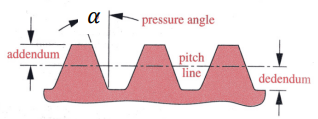
\includegraphics[scale=1]{Images/rack.png}
	\caption{Standard rack}
	\label{fig:rack}
\end{figure}\\
In our case we have:
\begin{equation*}
	\centering
	\alpha = 20\textdegree \Rightarrow z_{min} = 17,
\end{equation*}
that means that the interfence condition, in our project, is fulfilled because we designed a pinion with $z=18$.\\

\subsection{Tooth root fatigue resistance}
One of the most important problem in the usage of gears is the teeth fatigue resistance, due to the fact they're subjected to pulsating loads.\\
In our analysis we used the Lewis method that consider the tooth as a cantilever beam and shear and compressive normal stresses are neglected.\\
In order to compute the stress state we used the following equation:
\begin{equation}
	\centering
	\sigma_L=\frac{6F_t*h}{b*s_L^2},
	\label{stress}
\end{equation}
where $F_t$, $h$, $b$ and $s_L$ are showed in \figurename \ \ref{fig:tooth1} and \ref{fig:tooth2}.
\begin{figure}[hbt]
\begin{subfigure}{.5\textwidth}
	\centering
	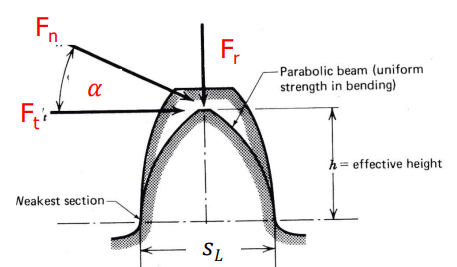
\includegraphics[scale=0.5]{Images/toothgear1.png}
	\caption{Tooth section}
	\label{fig:tooth1}
\end{subfigure}%
\begin{subfigure}{.5\textwidth}
	\centering
	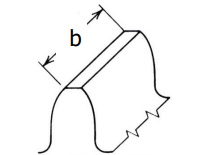
\includegraphics[scale=0.6]{Images/toothgear2.png}
	\caption{Face width}
	\label{fig:tooth2}
\end{subfigure}
\caption{Tooth details}
\end{figure}\\
In our project we used two motors with 10W 50rpm to actuate the machine. From this data we could find the actual force $F_t$ exerted on the teeth:
\begin{equation*}
	\centering
		T = \frac{P}{\omega} = \frac{10}{\frac{2\pi50}{60}} \ \frac{W}{rad/s} = 1.9 N*m 
\end{equation*}
\begin{equation*}
	\centering
	F_t = \frac{T}{r} = \frac{1.9}{17.14} \ \frac{W}{mm} = 111.3 N
\end{equation*}
At this point we can find the stress state, from \eqref{stress}:
\begin{equation}
	\centering
	\sigma_L=\frac{6*111.3*2.14}{10*1.79^2} = 44.6 MPa.
	\label{stressdata}
\end{equation}\\
The Lewis method provide the nominal stress state at the base of the tooth, in the hypothesis of considering the tooth as a cantilever beam.\\
All factors affecting the actual value of the stress state should therefore be taken into account in the design. Moreover, the admissible stress must be defined starting from the properties of the material and the production and processing techniques adopted.\\
